%----------------------------------------------------------------------------------------
%	PACKAGES AND OTHER DOCUMENT CONFIGURATIONS
%----------------------------------------------------------------------------------------

\documentclass[nobib, a4paper, notoc, oneside, openany]{tufte-book} % Use the tufte-book class which in turn uses the tufte-common class
% =============================================================================
% Tufte packages
% =============================================================================
% \hypersetup{colorlinks} % Comment this line if you don't wish to have colored links

\usepackage{microtype} % Improves character and word spacing

\usepackage{lipsum} % Inserts dummy text

\usepackage{booktabs} % Better horizontal rules in tables

\usepackage{graphicx} % Needed to insert images into the document
\graphicspath{{figures/}} % Sets the default location of pictures
\setkeys{Gin}{width=\linewidth,totalheight=\textheight,keepaspectratio} % Improves figure scaling

\usepackage{fancyvrb} % Allows customization of verbatim environments
\fvset{fontsize=\normalsize} % The font size of all verbatim text can be changed here

\usepackage{xspace} % Used for printing a trailing space better than using a tilde (~) using the \xspace command

\usepackage{units} % Used for printing standard units

\usepackage{makeidx} % Used to generate the index
\makeindex % Generate the index which is printed at the end of the document

% use the biblatex package
% \usepackage[style=authortitle-icomp, autocite=footnote, backend=biber]{biblatex}
\usepackage[style=numeric, autocite=footnote, backend=biber]{biblatex}
\addbibresource{bibliography.bib}

% =============================================================================
% My added packages
% =============================================================================
\usepackage[ngerman,american]{babel}

\usepackage{newfloat}
\usepackage{acronym}
\usepackage{url}

%minted Code-Environment
\usepackage{minted}
\setminted{
	fontsize=\footnotesize,
	breaklines,
	breakanywhere,
	linenos,
	numbersep=5pt,
	gobble=0,
	frame=single
}

\usepackage{lipsum}

\usepackage[disable]{todonotes}
% \usepackage{todonotes}

\usepackage[caption=false]{subfig}

\usepackage{amsmath}

\usepackage{appendix}
\usepackage{etoc}
\usepackage{etoolbox}

\usepackage{booktabs}

\usepackage{amssymb}

% =============================================================================
% Tufte definitions
% =============================================================================
\newcommand{\hangp}[1]{\makebox[0pt][r]{(}#1\makebox[0pt][l]{)}} % New command to create parentheses around text in tables which take up no horizontal space - this improves column spacing
\newcommand{\hangstar}{\makebox[0pt][l]{*}} % New command to create asterisks in tables which take up no horizontal space - this improves column spacing

\newcommand{\monthyear}{\ifcase\month\or January\or February\or March\or April\or May\or June\or July\or August\or September\or October\or November\or December\fi\space\number\year} % A command to print the current month and year

\newcommand{\openepigraph}[2]{ % This block sets up a command for printing an epigraph with 2 arguments - the quote and the author
\begin{fullwidth}
\sffamily\large
\begin{doublespace}
\noindent\allcaps{#1}\\ % The quote
\noindent\allcaps{#2} % The author
\end{doublespace}
\end{fullwidth}
}

\newcommand{\blankpage}{\newpage\hbox{}\thispagestyle{empty}\newpage} % Command to insert a blank page

\newcommand{\hlred}[1]{\textcolor{Maroon}{#1}} % Print text in maroon
\newcommand{\hangleft}[1]{\makebox[0pt][r]{#1}} % Used for printing commands in the index, moves the slash left so the command name aligns with the rest of the text in the index 
\newcommand{\hairsp}{\hspace{1pt}} % Command to print a very short space
\newcommand{\ie}{\textit{i.\hairsp{}e.}\xspace} % Command to print i.e.
\newcommand{\eg}{\textit{e.\hairsp{}g.}\xspace} % Command to print e.g.
\newcommand{\na}{\quad--} % Used in tables for N/A cells
\newcommand{\measure}[3]{#1/#2$\times$\unit[#3]{pc}} % Typesets the font size, leading, and measure in the form of: 10/12x26 pc.
\newcommand{\tuftebs}{\symbol{'134}} % Command to print a backslash in tt type in OT1/T1

\providecommand{\XeLaTeX}{X\lower.5ex\hbox{\kern-0.15em\reflectbox{E}}\kern-0.1em\LaTeX}
\newcommand{\tXeLaTeX}{\XeLaTeX\index{XeLaTeX@\protect\XeLaTeX}} % Command to print the XeLaTeX logo while simultaneously adding the position to the index

\newcommand{\doccmdnoindex}[2][]{\texttt{\tuftebs#2}} % Command to print a command in texttt with a backslash of tt type without inserting the command into the index

\newcommand{\doccmddef}[2][]{\hlred{\texttt{\tuftebs#2}}\label{cmd:#2}\ifthenelse{\isempty{#1}} % Command to define a command in red and add it to the index
{ % If no package is specified, add the command to the index
\index{#2 command@\protect\hangleft{\texttt{\tuftebs}}\texttt{#2}}% Command name
}
{ % If a package is also specified as a second argument, add the command and package to the index
\index{#2 command@\protect\hangleft{\texttt{\tuftebs}}\texttt{#2} (\texttt{#1} package)}% Command name
\index{#1 package@\texttt{#1} package}\index{packages!#1@\texttt{#1}}% Package name
}}

\newcommand{\doccmd}[2][]{% Command to define a command and add it to the index
\texttt{\tuftebs#2}%
\ifthenelse{\isempty{#1}}% If no package is specified, add the command to the index
{%
\index{#2 command@\protect\hangleft{\texttt{\tuftebs}}\texttt{#2}}% Command name
}
{%
\index{#2 command@\protect\hangleft{\texttt{\tuftebs}}\texttt{#2} (\texttt{#1} package)}% Command name
\index{#1 package@\texttt{#1} package}\index{packages!#1@\texttt{#1}}% Package name
}}

% A bunch of new commands to print commands, arguments, environments, classes, etc within the text using the correct formatting
\newcommand{\docopt}[1]{\ensuremath{\langle}\textrm{\textit{#1}}\ensuremath{\rangle}}
\newcommand{\docarg}[1]{\textrm{\textit{#1}}}
\newenvironment{docspec}{\begin{quotation}\ttfamily\parskip0pt\parindent0pt\ignorespaces}{\end{quotation}}
\newcommand{\docenv}[1]{\texttt{#1}\index{#1 environment@\texttt{#1} environment}\index{environments!#1@\texttt{#1}}}
\newcommand{\docenvdef}[1]{\hlred{\texttt{#1}}\label{env:#1}\index{#1 environment@\texttt{#1} environment}\index{environments!#1@\texttt{#1}}}
\newcommand{\docpkg}[1]{\texttt{#1}\index{#1 package@\texttt{#1} package}\index{packages!#1@\texttt{#1}}}
\newcommand{\doccls}[1]{\texttt{#1}}
\newcommand{\docclsopt}[1]{\texttt{#1}\index{#1 class option@\texttt{#1} class option}\index{class options!#1@\texttt{#1}}}
\newcommand{\docclsoptdef}[1]{\hlred{\texttt{#1}}\label{clsopt:#1}\index{#1 class option@\texttt{#1} class option}\index{class options!#1@\texttt{#1}}}
\newcommand{\docmsg}[2]{\bigskip\begin{fullwidth}\noindent\ttfamily#1\end{fullwidth}\medskip\par\noindent#2}
\newcommand{\docfilehook}[2]{\texttt{#1}\index{file hooks!#2}\index{#1@\texttt{#1}}}
\newcommand{\doccounter}[1]{\texttt{#1}\index{#1 counter@\texttt{#1} counter}}

% This block contains a number of shortcuts used throughout the book
\newcommand{\vdqi}{\textit{VDQI}\xspace}
\newcommand{\ei}{\textit{EI}\xspace}
\newcommand{\ve}{\textit{VE}\xspace}
\newcommand{\be}{\textit{BE}\xspace}
\newcommand{\VDQI}{\textit{The Visual Display of Quantitative Information}\xspace}
\newcommand{\EI}{\textit{Envisioning Information}\xspace}
\newcommand{\VE}{\textit{Visual Explanations}\xspace}
\newcommand{\BE}{\textit{Beautiful Evidence}\xspace}
\newcommand{\TL}{Tufte-\LaTeX\xspace}


% =============================================================================
% Modifications on Tufte layout
% =============================================================================
\titleclass{\subsubsection}{straight}
\titleformat{\chapter}%
  {\relax}% format applied to label+text
  {\itshape\huge\thechapter}% label
  {1em}% horizontal separation between label and title body
  {\huge\rmfamily\itshape}% before the title body
  []% after the title body

\titleformat{\subsubsection}%
  [hang]% shape
  {\normalfont\large\itshape}% format applied to label+text
  {\thesubsubsection}% label
  {1em}% horizontal separation between label and title body
  {}% before the title body
  []% after the title body

\setcounter{tocdepth}{2}
\setcounter{secnumdepth}{2}


% =============================================================================
% My definitions color
% =============================================================================
\definecolor{universityred}{RGB}{165,30,55}
\definecolor{black}{RGB}{0,0,0}

% basic color definitions
\definecolor{red}{RGB}{165, 30, 55} % #a51e37
\definecolor{blue}{RGB}{12, 48, 65} % #1e7ba5
\definecolor{light_blue}{RGB}{22, 66, 86} % #37a8db
\definecolor{yellow}{RGB}{65, 55, 12} % #a58c1e
\definecolor{light_yellow}{RGB}{86, 74, 22} % #dbbc37

\definecolor{chapterlink}{RGB}{165, 30, 55}


\hypersetup{
    colorlinks=true,
    linkcolor=chapterlink,
    urlcolor=light_blue,
    citecolor=yellow
    }

% =============================================================================
% Variable declarations
% =============================================================================
\def\authorsurname{Bar}
\def\authorfirstname{Foo}
\def\title{Title}
\def\thesiskind{Master's Thesis Computer Science}
\def\thesisstart{31.01.2024}
\def\thesisend{30.06.2024}

\def\namefirstsupervisor{Max Mustermann}
\def\facultyfirstsupervisor{Science}
\def\departmentfirstsupervisor{Computer Science}
\def\researchgroupfirstsupervisor{Neural Information Processing}

\def\namesecondsupervisor{Dr. John Smith}
\def\facultysecondsupervisor{Science}
\def\departmentsecondsupervisor{Lobortis}
\def\researchgroupsecondsupervisor{Ullamcorper suscipit}

% =============================================================================
% My definitions commands
% =============================================================================

% Anhang-Environment
\DeclareFloatingEnvironment[fileext=loAppend, listname={Appendix}, name=Appendix, placement=htbp]{append}
\renewcommand{\theappend}{\Alph{append}.}

% Code-Environment
\DeclareFloatingEnvironment[fileext=loCode, listname={Code}, name=Code, placement=htbp]{code}
% \renewcommand{\thecode}{\Alph{append}.}

% Linking commands (chapter, appendix)
\newcommand{\chapterref}[1]{Chapter \ref{#1}}
\newcommand{\figref}[1]{Figure \ref{#1}}
\newcommand{\tabref}[1]{Table \ref{#1}}
\newcommand{\appref}[1]{Appendix \ref{#1}}
\newcommand{\coderef}[1]{Code \ref{#1}}

% commands for appendix
\AtBeginEnvironment{appendix}{\etocsettocdepth.toc{chapter}\etocignoretoctocdepth}
\newcommand{\appsection}[1]{\clearpage\section{#1}}

%----------------------------------------------------------------------------------------

\begin{document}

\frontmatter

%----------------------------------------------------------------------------------------

% =============================================================================
% Titlepage
% =============================================================================
\newgeometry{top=2.7cm,left=2.5cm,right=2.5cm}
\begin{titlepage}
	\begin{adjustwidth}{0cm}{-1cm}
	\begin{minipage}{0.5\textwidth}
		
\includegraphics[width=\linewidth]{figures/logo.pdf}
	\end{minipage}
	\hfill
	\begin{minipage}{0.33\textwidth}
		{\bfseries\textsf{\textcolor{universityred}{Department of \departmentfirstsupervisor}}\\[0.3cm]}
		{\bfseries\textsf{\textcolor{universityred}{\researchgroupfirstsupervisor}}}
	\end{minipage}%
	\end{adjustwidth}
	\vspace{3cm}
	\begin{center}
		{\huge \thesiskind\\[2cm]}
		{\Large\bfseries \title\\[1.5cm]}
		{\large Submitted by: \authorfirstname\ \authorsurname}\\[0.5cm]
		\thesisend
	\end{center}
	\vfill
	\begin{minipage}{0.48\textwidth}
		\centering
		{\small\bfseries First Supervisor}\\[0.3cm]
		{\large \namefirstsupervisor}\\[2mm]
		{\footnotesize Faculty of \facultyfirstsupervisor\\
		Department of \departmentfirstsupervisor\\[1.5mm]
		\researchgroupfirstsupervisor\\
		University of Tübingen}
	\end{minipage}
	\hfill
	\begin{minipage}{0.48\textwidth}
		\centering
		{\small\bfseries Second Supervisor}\\[0.3cm]
		{\large \namesecondsupervisor}\\[2mm]
		{\footnotesize Faculty of \facultysecondsupervisor\\
		Department of \departmentsecondsupervisor\\[1.5mm]
		\researchgroupsecondsupervisor\\
		University of Tübingen}
	\end{minipage}%
	\vspace{1.5cm}
\end{titlepage}
\restoregeometry
\vspace*{\fill}
\noindent
\begin{minipage}{.8\textwidth}
	\textbf{\authorsurname, \authorfirstname:}\\
	\emph{\title}\\
	\thesiskind\\
	University of Tübingen\\
	Processing period: \thesisstart\ - \thesisend
\end{minipage}

%----------------------------------------------------------------------------------------

%----------------------------------------------------------------------------------------
%	Abstract
%----------------------------------------------------------------------------------------
\chapter{Abstract}
\begin{fullwidth}
Lorem ipsum dolor sit amet, consetetur sadipscing elitr, sed diam nonumy eirmod tempor invidunt ut labore et dolore magna aliquyam erat, sed diam voluptua. At vero eos et accusam et justo duo dolores et ea rebum. Stet clita kasd gubergren, no sea takimata sanctus est Lorem ipsum dolor sit amet. Lorem ipsum dolor sit amet, consetetur sadipscing elitr, sed diam nonumy eirmod tempor invidunt ut labore et dolore magna aliquyam erat, sed diam voluptua. At vero eos et accusam et justo duo dolores et ea rebum. Stet clita kasd gubergren, no sea takimata sanctus est Lorem ipsum dolor sit amet. Lorem ipsum dolor sit amet, consetetur sadipscing elitr, sed diam nonumy eirmod tempor invidunt ut labore et dolore magna aliquyam erat, sed diam voluptua. At vero eos et accusam et justo duo dolores et ea rebum. Stet clita kasd gubergren, no sea takimata sanctus est Lorem ipsum dolor sit amet.   

Duis autem vel eum iriure dolor in hendrerit in vulputate velit esse molestie consequat, vel illum dolore eu feugiat nulla facilisis at vero eros et accumsan et iusto odio dignissim qui blandit praesent luptatum zzril delenit augue duis dolore te feugait nulla facilisi. Lorem ipsum dolor sit amet, consectetuer adipiscing elit, sed diam nonummy nibh euismod tincidunt ut laoreet dolore magna aliquam erat volutpat.   

Ut wisi enim ad minim veniam, quis nostrud exerci tation ullamcorper suscipit lobortis nisl ut aliquip ex ea commodo consequat. Duis autem vel eum iriure dolor in hendrerit in vulputate velit esse molestie consequat, vel illum dolore eu feugiat nulla facilisis at vero eros et accumsan et iusto odio dignissim qui blandit praesent luptatum zzril delenit augue duis dolore te feugait nulla facilisi.   

Nam liber tempor cum soluta nobis eleifend option congue nihil imperdiet doming id quod mazim placerat facer possim assum. Lorem ipsum dolor sit amet, consectetuer adipiscing elit, sed diam nonummy nibh euismod tincidunt ut laoreet dolore magna aliquam erat volutpat. Ut wisi enim ad minim veniam, quis nostrud exerci tation ullamcorper suscipit lobortis nisl ut aliquip ex ea commodo
\end{fullwidth}

\begin{fullwidth}
% \parttoc % Insert the document TOC
\etocsettocdepth{subsection}
\tableofcontents % Print the table of contents
% redefine the headings of the TOCs to use \section* rather than \chapter*
\etocarticlestyle
\end{fullwidth}

\mainmatter

%----------------------------------------------------------------------------------------
%	INTRODUCTION
%----------------------------------------------------------------------------------------
\chapter{Introduction}
This is an example chapter that uses commands specific to the tufte layout and the created commands. The commands were developed during the writing of \cite{schmiegel2023}. That master thesis was written in the \ac{nip} research group.

\section{Vero Eos}
At vero eos et accusam et justo duo dolores et ea rebum. Stet clita kasd gubergren, no sea takimata sanctus est Lorem ipsum dolor sit amet. 

\begin{marginfigure}
    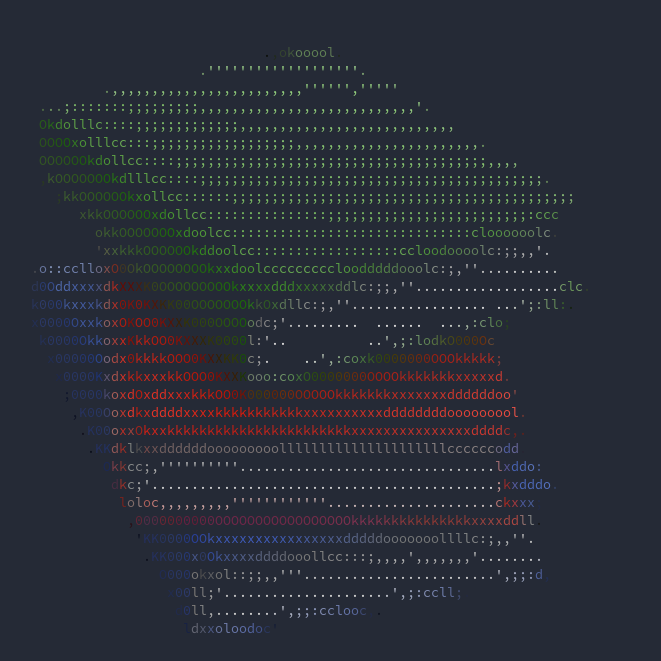
\includegraphics{figures/books.png}
    \caption{Lorem ipsum dolor sit amet. More information about the image can be found in \protect\appref{app:appendix3}.}
    \label{fig:books}
\end{marginfigure}

Lorem ipsum dolor sit amet, consetetur sadipscing elitr, sed diam nonumy eirmod tempor invidunt ut labore et dolore magna aliquyam erat, sed diam voluptua. At vero eos et accusam et justo duo dolores et ea rebum.\footnote{Duis autem vel eum iriure dolor in hendrerit.} Stet clita kasd gubergren, no sea takimata sanctus est Lorem ipsum dolor sit amet. Lorem ipsum dolor sit amet, consetetur sadipscing elitr, sed diam nonumy eirmod tempor invidunt ut labore et dolore magna aliquyam erat, sed diam voluptua.\footnote{Augue duis dolore te.} At vero eos et (\coderef{code:pyem2a}) accusam et justo duo dolores et ea rebum. Stet clita kasd gubergren, no sea takimata sanctus est Lorem ipsum dolor sit amet.

\begin{code}
\begin{minted}[breaklines, breakanywhere, linenos, numbersep=5pt, gobble=0, frame=leftline]{python}
def extractEmojis(unicode):
    global fileName
    # test if file already exists
    fileName = f'./images/{unicode}.png'
    file_exists = os.path.exists(fileName)
    if not file_exists:
        # download emoji
        url = f'https://emoji.aranja.com/static/emoji-data/img-apple-160/{unicode}.png'
        urllib.request.urlretrieve(url, fileName)
\end{minted}
\caption{This code is part of the pyem2a project.}
\label{code:pyem2a}
\end{code}

\subsection{Eum Iriure Dolor}
Duis autem vel eum iriure dolor in hendrerit in vulputate velit esse molestie consequat, vel illum dolore eu feugiat nulla facilisis at vero eros et accumsan et iusto odio dignissim qui blandit praesent luptatum zzril delenit augue duis dolore te feugait nulla facilisi.\footnote{Stet clita kasd gubergren, no sea takimata sanctus est Lorem ipsum dolor sit amet.} Lorem ipsum dolor sit amet, consectetuer adipiscing elit, sed diam nonummy nibh euismod tincidunt ut laoreet dolore magna aliquam erat (\figref{fig:books2}) volutpat.

\begin{figure}
    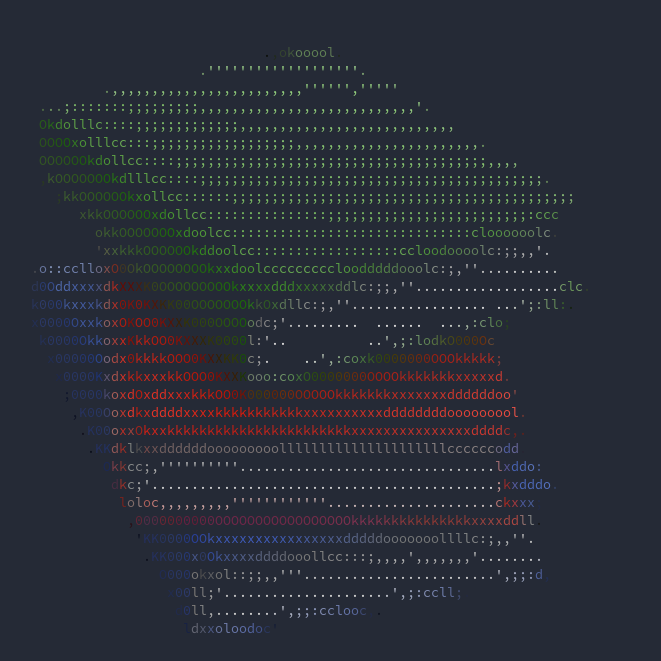
\includegraphics{figures/books.png}
    \caption[Lorem ipsum dolor sit amet.]{Lorem ipsum dolor sit amet. More information about the image can be found in \appref{app:appendix3}.}
    \label{fig:books1}
\end{figure}

\subsection{Minim Veniam}
Ut wisi enim ad minim veniam, quis nostrud exerci tation ullamcorper suscipit lobortis nisl ut aliquip ex ea commodo consequat. Duis autem vel eum iriure dolor in hendrerit in vulputate velit esse molestie consequat, vel illum dolore eu feugiat nulla facilisis at vero eros et accumsan et iusto odio dignissim qui blandit praesent luptatum zzril delenit augue duis dolore te feugait nulla facilisi.

Nam liber tempor cum soluta nobis eleifend option congue nihil imperdiet doming id quod mazim placerat facer possim assum. Lorem ipsum dolor sit amet, consectetuer adipiscing elit, sed diam nonummy nibh euismod tincidunt ut laoreet dolore magna aliquam erat volutpat. Ut wisi enim ad minim veniam, quis nostrud exerci tation ullamcorper suscipit lobortis nisl ut aliquip ex ea commodo consequat.

Duis autem vel eum iriure dolor in hendrerit in vulputate velit esse molestie consequat, vel illum dolore eu feugiat nulla facilisis.

\begin{figure*}
    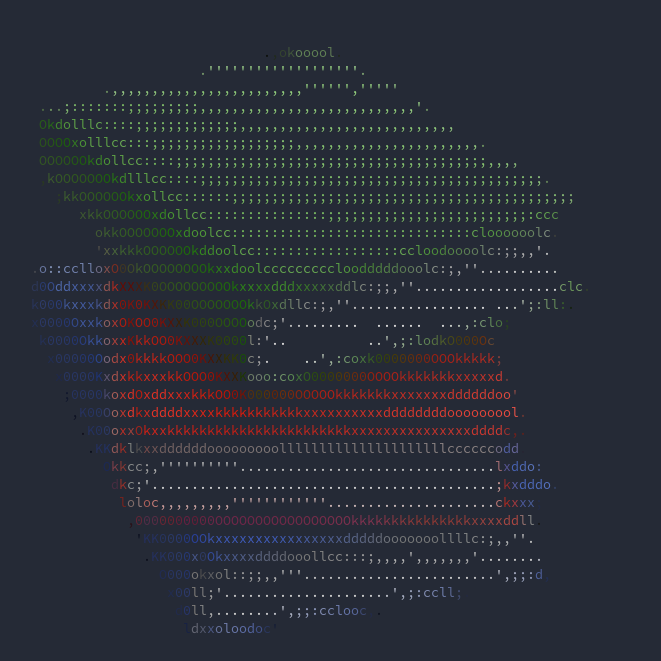
\includegraphics[width=15cm]{figures/books.png}
    \caption[Lorem ipsum dolor sit amet.]{Lorem ipsum dolor sit amet. More information about the image can be found in \appref{app:appendix3}.}
    \label{fig:books2}
\end{figure*}

\section{Sed Diam Voluptua}
Lorem ipsum dolor sit amet, consetetur sadipscing elitr, sed diam nonumy eirmod tempor invidunt ut labore et dolore magna aliquyam erat, sed diam voluptua. At vero eos et accusam et justo duo dolores et ea rebum. Stet clita kasd gubergren, no sea takimata sanctus est Lorem ipsum dolor sit amet. Lorem ipsum dolor sit amet, consetetur sadipscing elitr, sed diam nonumy eirmod tempor invidunt ut labore et dolore magna aliquyam erat, sed diam voluptua. At vero eos et accusam et justo duo dolores et ea rebum. Stet clita kasd gubergren, no sea takimata sanctus est Lorem ipsum dolor sit amet. Lorem ipsum dolor sit amet, consetetur sadipscing elitr, sed diam nonumy eirmod tempor invidunt ut labore et dolore magna aliquyam erat, sed diam voluptua. At vero eos et accusam et justo duo dolores et ea rebum. Stet clita kasd gubergren, no sea takimata sanctus est Lorem ipsum dolor sit amet.\footnote{For more information see \tabref{tab:table1}}

\begin{table}[ht]
    \centering
    \begin{tabular}{@{}lll@{}}
    \toprule
    \textbf{name} & \textbf{value 1} & \textbf{value 2} \\ 
    \midrule
    zzril delenit & 1.000 & 0.119838 \\
    option congue & 5.000 & 0.347119 \\
    imperdiet doming & 0.125 & 0.404985 \\
    id quod & 1.375 & 0.358990 \\
    mazim placerat & 0.125 & 0.116606 \\
    sed diam & 0.500 & 0.219490 \\
    minim veniam & 0.625 & 0.112587 \\
    \bottomrule
    \end{tabular}
    \caption{An example for a table}
    \label{tab:table1}
\end{table}


Duis autem vel eum iriure dolor in hendrerit in vulputate velit esse molestie consequat, vel illum dolore eu feugiat nulla facilisis at vero eros et accumsan et iusto odio dignissim qui blandit praesent luptatum zzril delenit augue duis dolore te feugait nulla facilisi.

\begin{table*}
    \centering
    \begin{tabular}{llllllll}
        \toprule
        \textbf{feugait} & \textbf{dolore} & \textbf{odio} & \textbf{prior} & \textbf{iusto} & \textbf{feugait} & \textbf{praesent} & \textbf{et} \\
        \midrule
        Lorem & Ipsum & Dolor & & adipiscing & (1, 1) & hendrerit & [[101.6995]] \\
        facilisis & Ipsum & Dolor & & adipiscing & (1,) & hendrerit & [-4.14673] \\
        Dolor & Ipsum & Dolor & & Lorem & () & hendrerit & 2.68172 \\
        Ipsum & diam & Ipsum & & euismod & () & hendrerit & 95.24376 \\
        Ipsum & euismod & kasd & & sed & () & hendrerit & 0.44245 \\
        nonummy & Ipsum & Ipsum & & volutpat & () & hendrerit & 578.3492 \\
        Ipsum & sed & Dolor & & volutpat & () & hendrerit & 17.7574 \\
        Ipsum & Ipsum & diam & & aliquam & (1, 1) & hendrerit & [[0.31899]] \\
        Ipsum & Ipsum & Dolor & & dolore & (1,) & hendrerit & [2.67118] \\
        \bottomrule
    \end{tabular}
    \caption[][0.4cm]{Stet clita kasd gubergren, no sea takimata sanctus est Lorem ipsum dolor sit amet.}
    \label{tab:table2}
\end{table*}

Lorem ipsum dolor sit amet,\sidenote[][1cm]{See \tabref{tab:table2}.} consectetuer adipiscing elit, sed diam nonummy nibh euismod tincidunt ut laoreet dolore magna aliquam erat volutpat.   

\begin{figure*}
    \centering
    \subfloat[subtitle 1]{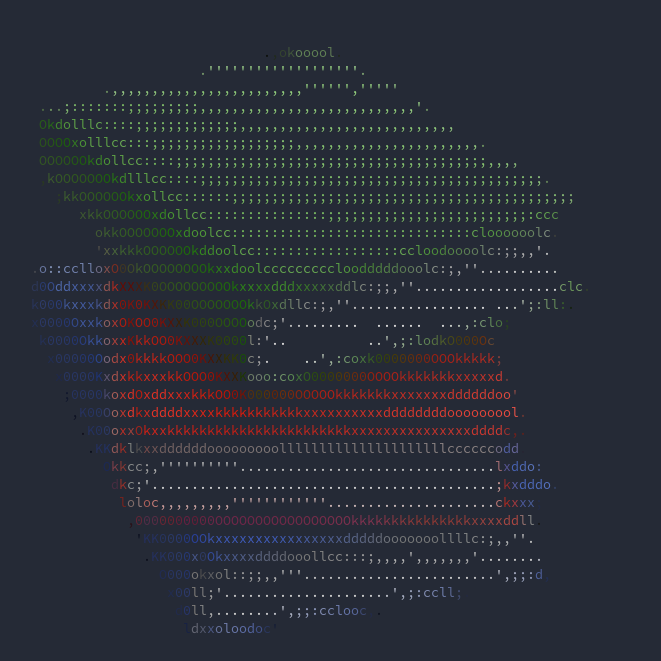
\includegraphics[width=0.45\textwidth]{figures/books.png}}
    \hfill
    \subfloat[subtitle 2]{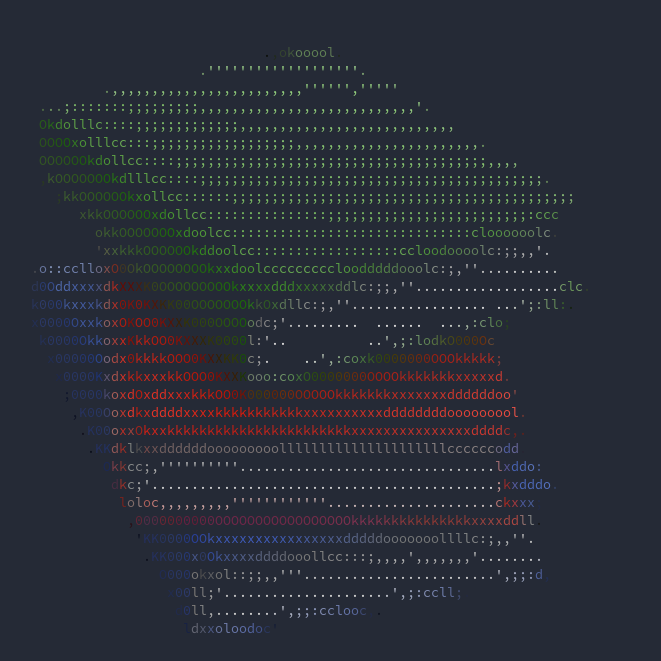
\includegraphics[width=0.45\textwidth]{figures/books.png}}
    \vspace{0.5cm}
    \caption{Duis autem vel eum iriure dolor in hendrerit.\label{fig:ComparisonWithGammaDetailed}}
\end{figure*}

Ut wisi enim ad minim veniam, quis nostrud exerci tation ullamcorper suscipit lobortis nisl ut aliquip ex ea commodo consequat. Duis autem vel eum iriure dolor in hendrerit in vulputate velit esse molestie consequat, vel illum dolore eu feugiat nulla facilisis at vero eros et accumsan et iusto odio dignissim qui blandit praesent luptatum zzril delenit augue duis dolore te feugait nulla facilisi.   

Nam liber tempor cum soluta nobis eleifend option congue nihil imperdiet doming id quod mazim placerat facer possim assum. Lorem ipsum dolor sit amet, consectetuer adipiscing elit, sed diam nonummy nibh euismod tincidunt ut laoreet dolore magna aliquam erat volutpat. Ut wisi enim ad minim veniam, quis nostrud exerci tation ullamcorper suscipit lobortis nisl ut aliquip ex


%----------------------------------------------------------------------------------------
%	CHAPTER 2 ....
%----------------------------------------------------------------------------------------
% \input{chapters/filename}

%----------------------------------------------------------------------------------------

\backmatter

%----------------------------------------------------------------------------------------
%	BIBLIOGRAPHY
%----------------------------------------------------------------------------------------

\begin{fullwidth}
	\printbibliography
	\addcontentsline{toc}{chapter}{Bibliography}
\end{fullwidth}

%----------------------------------------------------------------------------------------

% Abbreviations
\chapter*{List of Abbreviations} \label{ch:Abbreviations}
\addcontentsline{toc}{chapter}{List of Abbreviations}
\begin{acronym}
    \acro{nip}[NIP]{Neural Information Processing}
\end{acronym}

%----------------------------------------------------------------------------------------
\makeatletter
\renewcommand*\l@figure{\@dottedtocline{1}{1.5em}{2.3em}}
\makeatother
\begin{fullwidth}
	\listoffigures % Print a list of figures
	\addcontentsline{toc}{chapter}{List of Figures}
\end{fullwidth}

%----------------------------------------------------------------------------------------
\makeatletter
\renewcommand*\l@code{\@dottedtocline{1}{1.5em}{2.3em}}
\makeatother
\begin{fullwidth}
	\listofcode % Print a list of Code
	\addcontentsline{toc}{chapter}{List of Code}
\end{fullwidth}

%----------------------------------------------------------------------------------------

\makeatletter
\renewcommand*\l@table{\@dottedtocline{1}{1.5em}{2.3em}}
\makeatother
\begin{fullwidth}
	\listoftables % Print a list of tables
	\addcontentsline{toc}{chapter}{List of Tables}
\end{fullwidth}

%----------------------------------------------------------------------------------------
%	Appendix
%----------------------------------------------------------------------------------------
\appendix
\begin{appendix}
\input{appendix/appendix.tex}
\end{appendix}

% =============================================================================
% "I did this myself"
% =============================================================================
\begin{otherlanguage}{german}
\begin{fullwidth}
    \chapter*{Selbstständigkeitserklärung}
    Hiermit erkläre ich, dass ich diese schriftliche Abschlussarbeit selbständig verfasst habe, keine anderen als die angegebenen Hilfsmittel und Quellen benutzt habe und alle wörtlich oder sinngemäß aus anderen Werken übernommenen Aussagen als solche gekennzeichnet habe.
\end{fullwidth}
\vskip 3cm
Ort, Datum	\hfill Unterschrift
\end{otherlanguage}
% =============================================================================


\end{document}